\documentclass{midl} % Include author names
%\documentclass[anon]{midl} % Anonymized submission

% The following packages will be automatically loaded:
% jmlr, amsmath, amssymb, natbib, graphicx, url, algorithm2e
% ifoddpage, relsize and probably more
% make sure they are installed with your latex distribution

\usepackage{mwe} % to get dummy images
%\usepackage{tabularx}
\usepackage{algorithm}
\usepackage{algpseudocode}
\usepackage{multirow}
\usepackage{float}
\usepackage{wrapfig}
\usepackage{color,soul}
\usepackage{comment}
\usepackage{graphicx}
\usepackage{booktabs}
%\jmlrvolume{-- Under Review}
\jmlryear{2023}
\jmlrworkshop{Report for final exam}
%\editors{Knowledge Discovery Course - UNICT}
\usepackage{hyperref} % For URL linking
\hypersetup{
    colorlinks=true,
    linkcolor=blue,
    urlcolor=blue,
    citecolor=blue
}
\usepackage{lipsum} % For dummy text


\title[Exploring the Effects of Perturbed and Adversarial Dreaming]{Exploring the Effects of Perturbed and Adversarial Dreaming on Learning Cortical Representations: A Replication Study of 'Learning Cortical Representations Through Perturbed and Adversarial Dreaming'} 

 % Use \Name{Author Name} to specify the name.
 % If the surname contains spaces, enclose the surname
 % in braces, e.g. \Name{John {Smith Jones}} similarly
 % if the name has a "von" part, e.g \Name{Jane {de Winter}}.
 % If the first letter in the forenames is a diacritic
 % enclose the diacritic in braces, e.g. \Name{{\'E}louise Smith}

 % Two authors with the same address
 % \midlauthor{\Name{Author Name1} \Email{abc@sample.edu}\and
 %  \Name{Author Name2} \Email{xyz@sample.edu}\\
 %  \addr Address}

 % Three or more authors with the same address:
 % \midlauthor{\Name{Author Name1} \Email{an1@sample.edu}\\
 %  \Name{Author Name2} \Email{an2@sample.edu}\\
 %  \Name{Author Name3} \Email{an3@sample.edu}\\
 %  \addr Address}


% Authors with different addresses:
% \midlauthor{\Name{Author Name1} \Email{abc@sample.edu}\\
% \addr Address 1
% \AND
% \Name{Author Name2} \Email{xyz@sample.edu}\\
% \addr Address 2
% }

%\footnotetext[1]{Contributed equally}

% More complicate cases, e.g. with dual affiliations and joint authorship
\midlauthor{\Name{Thamires de Souza Oliveira} \Email{thasouzaoliv@gmail.com}}
\begin{document}
\maketitle


\section{The Article}
The purpose of this report is to replicate and investigate the findings presented in an academic article, which can be accessed through the following link: \url{https://elifesciences.org/articles/76384}.

\subsection{Objective}
The primary objective of the article is to propose a new functional model of cortical representation learning, which posits that dreams, specifically their creative development of episodic memories, play a fundamental role in the formation of semantic representations during the evolutionary process. The authors introduce a cortical architecture inspired by generative adversarial networks (GANs) and train the model using established datasets of natural images to assess the quality of the acquired representations. The research aims to offer insights into the processing and representation of sensory experiences in the brain, with potential implications for comprehending the mechanisms through which humans and other organisms learn from sensory input.

\subsection{Dreams and Semantic Representations}
The article puts forth the notion that dreams, particularly their ability to combine diverse memories, are pivotal for the development of meaningful knowledge within the brain. This knowledge is stored as semantic representations, which distill pertinent information from sensory experiences while disregarding extraneous details, thereby facilitating their utilization across various brain regions.

\subsection{Semantic Representation Formation}
To support this proposition, the authors propose a inovative model elucidating how the brain learns and constructs these semantic representations. The model entails a creative process in which information flows from higher to lower brain areas, analogous to the occurrence of dreaming during rapid eye movement (REM) sleep. This process seeks to generate new but plausible sensory experiences by deceiving the brain's internal mechanisms that distinguish between wakefulness and REM sleep.

By generating fresh sensory experiences instead of merely reconstructing past observations, the brain is compelled to comprehend the composition of its sensory input. This perspective aligns with the notion that cortical representations, the neural patterns in the outer layer of the brain, should encapsulate meaningful and abstracted information rather than being tethered to specific contexts or details.


\section{Network Structure}

The network structure in this study comprises two primary components: the encoder/discriminator pathway and the generator pathway. Let's explore each component in detail:

\subsection{Encoder/Discriminator Pathway}
\begin{itemize}
  \item The encoder (Ez) takes input pixel data and maps it to a latent space.
  \item Ez consists of four convolutional layers, each with a different number of channels: 64, 128, 256, and 256.
  \item Each convolutional layer utilizes a 4x4 kernel, a stride of 2, and a LeakyReLU nonlinearity.
  \item The feature size is reduced by half in each layer.
  \item The output of the encoder's last convolutional layer is denoted as "z."
  \item An additional convolutional layer followed by a sigmoid nonlinearity is added on top of the second-to-last layer.
  \item This layer maps to a single scalar value "d," representing internal/external discrimination.
  \item The mapping from input data "x" to "d" is referred to as Ed.
  \item The first three convolutional layers are shared between Ez and Ed.
\end{itemize}

\subsection{Generator Pathway}
\begin{itemize}
  \item The generator (G) takes data from the latent space and maps it back to the pixel space.
  \item G consists of four deconvolutional layers with different numbers of channels: 256, 128, 64, and 3.
  \item Each deconvolutional layer employs a 4x4 kernel, a stride of 2, and either a LeakyReLU or tanh nonlinearity.
  \item The feature size is doubled in each layer.
  \item The output of the generator represents the reconstructed pixel data.
\end{itemize}

To summarize, the encoder/discriminator pathway (E) involves Ez, responsible for encoding pixel data to the latent space, and Ed, which performs discrimination. The generator pathway (G) maps data from the latent space back to the pixel space. Both pathways share the first three convolutional layers, with the encoder incorporating an additional layer for discrimination. The generator consists of four deconvolutional layers followed by appropriate non-linearities and aims to reconstruct the pixel data.



\section{The Datasets}

The model used in this study was trained on four standard datasets of natural images, namely:

\subsection{CIFAR-10 (Canadian Institute for Advanced Research 10)}
\begin{itemize}
  \item Composition: CIFAR-10 consists of a collection of 60,000 color images categorized into 10 different classes, with 6,000 images per class.
  \item Classes: The dataset covers a range of objects, including airplanes, automobiles, birds, cats, deer, dogs, frogs, horses, ships, and trucks.
  \item Image Size: Each image in CIFAR-10 has a resolution of 32x32 pixels.
  \item Training and Test Sets: The dataset is split into a training set containing 50,000 images and a test set containing 10,000 images, with an equal distribution of classes in both sets.
  \item Usage: CIFAR-10 is commonly utilized as a benchmark dataset for evaluating image classification algorithms and serves as a standard reference for machine learning tasks.
\end{itemize}

\subsection{SVHN (Street View House Numbers)}
\begin{itemize}
  \item Composition: SVHN comprises real-world images of house numbers extracted from Google Street View images.
  \item Classes: The primary focus of the dataset is recognizing and localizing digits ranging from 0 to 9.
  \item Image Size: The images in SVHN exhibit varying sizes and aspect ratios, generally higher in resolution compared to CIFAR-10 and MNIST.
  \item Training, Validation, and Test Sets: SVHN provides three distinct sets: a training set with approximately 73,257 images, a validation set with around 26,032 images, and a test set with roughly 26,032 images.
  \item Usage: SVHN is widely employed for tasks involving digit recognition, object localization, and multi-digit recognition.
\end{itemize}

\subsection{MNIST (Modified National Institute of Standards and Technology)}
\begin{itemize}
  \item Composition: MNIST consists of a collection of handwritten digit images sourced from multiple contributors.
  \item Classes: The dataset comprises images representing digits ranging from 0 to 9.
  \item Image Size: Each image in MNIST has a resolution of 28x28 pixels and is presented in grayscale.
  \item Training, Validation, and Test Sets: MNIST provides a training set with 60,000 images and a separate test set containing 10,000 images. Although a dedicated validation set is not included, researchers often create one by partitioning the training set.
  \item Usage: MNIST is widely recognized as a fundamental dataset for training and evaluating models in the field of machine learning, particularly in tasks related to handwritten digit recognition.
\end{itemize}

\subsection{Fashion MNIST}
\begin{itemize}
  \item Composition: Fashion MNIST was specifically developed as a drop-in replacement for MNIST, featuring fashion-related images.
  \item Classes: The dataset encompasses images of various fashion items, such as T-shirts, trousers, pullovers, dresses, coats, sandals, shirts, sneakers, bags, and ankle boots.
  \item Image Size: Each image in Fashion MNIST has a resolution of 28x28 pixels and is presented in grayscale.
  \item Training and Test Sets: Similar to MNIST, Fashion MNIST offers a training set consisting of 60,000 images and a test set containing 10,000 images. Researchers have the flexibility to create a validation set by splitting the training set.
  \item Usage: Fashion MNIST serves as an alternative to MNIST and is commonly utilized to evaluate and compare machine learning models specifically in the domain of fashion-related image classification.
\end{itemize}

\section{Training}

During the training process, the following key aspects were considered:

\begin{enumerate}
  \item Optimization Algorithm: We employ the ADAM optimizer, a popular choice in deep learning. ADAM utilizes adaptive learning rates and momentum to effectively update the model's parameters, ensuring efficient convergence during training.

  \item Learning Rate: The learning rate governs the step size taken when updating the model's parameters. We set the learning rate to 0.0002, which controls the magnitude of parameter adjustments made in each iteration, striking a balance between rapid convergence and fine-grained parameter updates.

  \item Mini-Batch Size: To optimize efficiency and leverage parallel processing capabilities, we adopt a mini-batch training approach. This involves performing parameter updates based on subsets, or mini-batches, of the training data. We choose a mini-batch size of 64, indicating that gradients are computed and parameters are updated using 64 samples at a time.

  \item Condition-Specific Objective Functions: We tailor specific loss functions for different conditions or tasks within the model. These loss functions quantify the discrepancy between the model's predictions and the desired outputs for each condition. By customizing the objective functions, we can effectively optimize the model's performance on specific tasks.

  \item Fully Differentiable Model: The model architecture is designed to ensure differentiability for all operations. This means that gradients can be computed for all parameters using backpropagation, facilitating efficient optimization of the model's parameters through gradient-based methods like stochastic gradient descent (SGD). The differentiability property enables smooth and effective updates to the model's parameters during training.
\end{enumerate}

In summary, the training approach utilizes stochastic gradient descent with mini-batches. We employ the ADAM optimizer with a learning rate of 0.0002 and a mini-batch size of 64. The model incorporates condition-specific loss functions, allowing it to be optimized for different tasks. Additionally, the model's architecture guarantees full differentiability, enabling efficient parameter updates during training.



\section{Creation of Samples}

In this study, the training and evaluation of a Generative Adversarial Network (GAN) model were facilitated for the purpose of generating realistic images. The GAN architecture consisted of two primary components: the generator and the discriminator.

The generator component accepted random noise as input and produced synthetic images. During the training phase, the generator learned to generate images that closely resembled the real training data by minimizing the discrepancy between its generated images and the real images.

Conversely, the discriminator functioned as a binary classifier with the objective of distinguishing between real and generated images. Through training, the discriminator was taught to correctly classify real images as genuine and generated images as fake.

To create a set of samples, the generator was employed to produce synthetic images by inputting random noise. These synthetic images were not part of the original training dataset but were generated using the trained generator model. By generating multiple samples, a collection of synthetic images was obtained, representing diverse outputs from the generator.


The following samples were included in the dataset:



\textbf{Sample 1: 'eval\_wake1\_000.png'}
This image serves as an evaluation sample derived from the first batch. It likely represents a sample of data captured during a wakeful state. The specific content and characteristics of this image would depend on the context and the dataset from which it originated.
The following image is a sample generated from the svhn dataset:

\begin{center}
    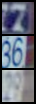
\includegraphics[width=0.15\textwidth]{eval_wake1_000.png}
    % Adjust the width as per your desired size
\end{center}

\textbf{Sample 2: 'eval\_wake2\_000.png'}
This image represents an evaluation sample from the second batch. Similar to the previous image, it signifies a sample obtained during a wakeful state. However, it pertains to a different batch, and variations between 'eval\_wake1\_000.png' and 'eval\_wake2\_000.png' may arise due to differences in the data or temporal aspects. The following image is a sample generated from the cifar10 dataset:
\begin{center}
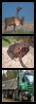
\includegraphics[width=0.15\textwidth]{eval_wake2_000.png}\hfill
% Add the path to 'eval_wake2_000.png' above
\end{center}

\textbf{Sample 3: 'eval\_nrem.png'}
This image corresponds to a generated sample that aims to depict the Non-REM (NREM) stage of sleep. Non-REM sleep is characterized by slow brain waves, reduced muscle activity, and deep sleep. The generated image likely encapsulates features or patterns associated with this specific sleep stage. The following image is a sample generated from the fashion dataset:
\begin{center}
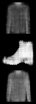
\includegraphics[width=0.15\textwidth]{eval3_nrem.png}\hfill
\end{center}
% Add the path to 'eval_nrem.png' above

\textbf{Sample 4: 'eval\_rem.png'}
This image represents a generated sample intended to capture the Rapid Eye Movement (REM) stage of sleep. REM sleep is characterized by vivid dreaming, rapid eye movements, and heightened brain activity. The generated image likely encompasses elements or patterns that typify this particular stage of sleep. The following image is a sample generated from the mnist dataset:
\begin{center}

\includegraphics[width=0.15\textwidth]{eval3_rem.png}
% Add the path to 'eval_rem.png' above
\end{center}

All the samples created can be found \href{https://drive.google.com/drive/folders/1ICiG1oI5mtNa3IMUPqH2Jn6dpg38qHH3}{here}.


\section{Evaluation Procedure}

The evaluation of the trained model involves some metrics and techniques to assess its performance and characteristics. Here are the key points explained in a clear and concise manner:

\begin{enumerate}
  \item Linear Classifier Training: A linear classifier is trained using the latent features (Z) extracted from the training dataset images. The classifier employs a weight matrix (W) to project the latent features onto label neurons and generate predictions.

  \item Loss Function: The classifier is trained using a multiclass cross-entropy loss function, which measures the difference between the predicted class probabilities and the target class.

  \item Occluded Data Evaluation: To assess the model's performance on occluded data, random square occlusion masks are applied to the test samples. The occlusion size remains fixed at 4. Results are reported for different levels of occlusion probability.
 
 \item The provided code involves training a linear classifier using latent variables. Despite unsupervised learning, the confusion matrix is applicable here for evaluating the classifier's performance in predicting labels. By comparing true and predicted labels, the confusion matrix provides insights into classification accuracy.
\end{enumerate}

\subsection{Evaluation - CIFAR10}
\subsubsection{Linear Classification}
\begin{figure} [H]
  \centering
  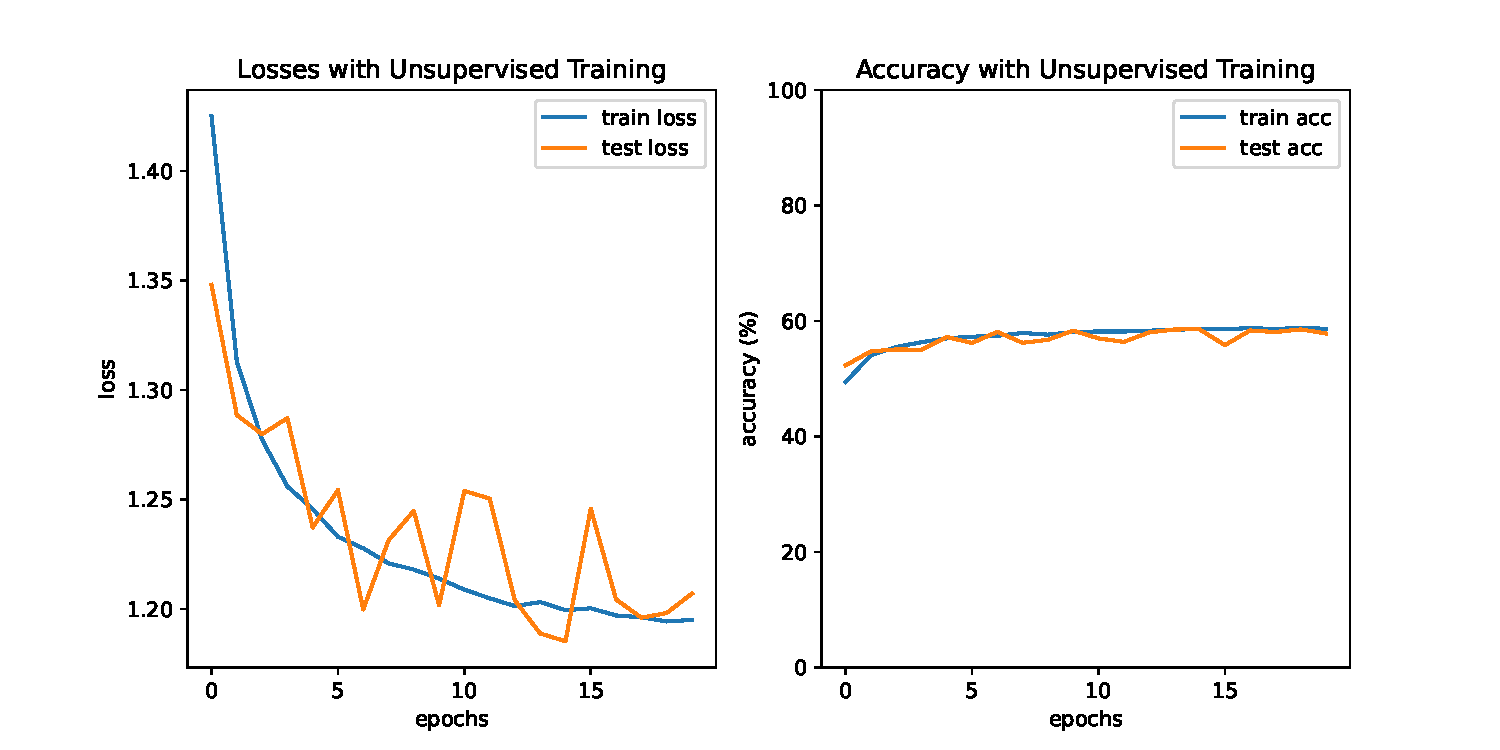
\includegraphics[width=1.2\textwidth]{linear_classif_cifar10.pdf}
  \caption{linear classification - cifar10}
  \label{fig:linear classification - cifar10}
\end{figure}

The observed patterns in the graph suggest that the model is gradually improving its predictions on the training data, as indicated by the steady decrease in train loss over epochs. However, the test loss shows fluctuations, indicating that the model may struggle to generalize well to unseen data. The train and test accuracies start around 50\% and increase to approximately 58\%, suggesting that the model performs slightly better than random guessing but has room for improvement.

\subsubsection{Losses}
\begin{figure}[ht]
  \centering
  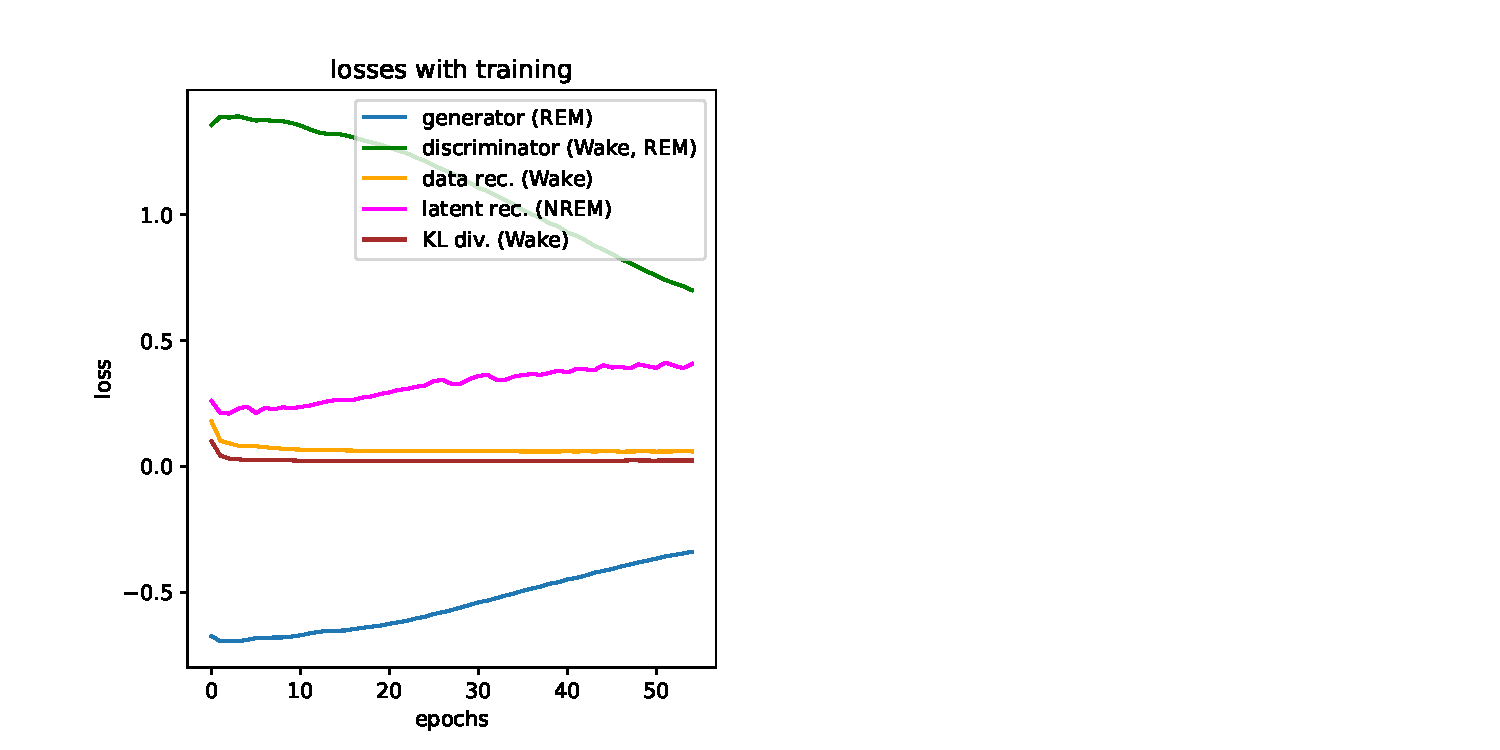
\includegraphics[width=1.2\textwidth]{losses_cifar10.pdf}
  \caption{losses - cifar10}
  \label{fig:losses - cifar10}
\end{figure}

The graph consists of two subplots. The first subplot displays the losses during training. The generator loss (associated with REM sleep) initially increases but starts to rise more sharply after 20 epochs. The discriminator loss (associated with both Wake and REM sleep) starts at 1.5 and gradually decreases over time. The losses for data reconstruction (Wake) and latent reconstruction (NREM) remain relatively stable, slightly above 0.0.

These patterns suggest that the generator's performance deteriorates over time, potentially indicating a challenge in generating high-quality samples. On the other hand, the discriminator shows improved discrimination ability as its loss decreases. The stable losses for data and latent reconstruction suggest that the model is maintaining consistency in reconstructing the input data.


\subsubsection{Occlusions}
\begin{figure}[H]
  \centering
  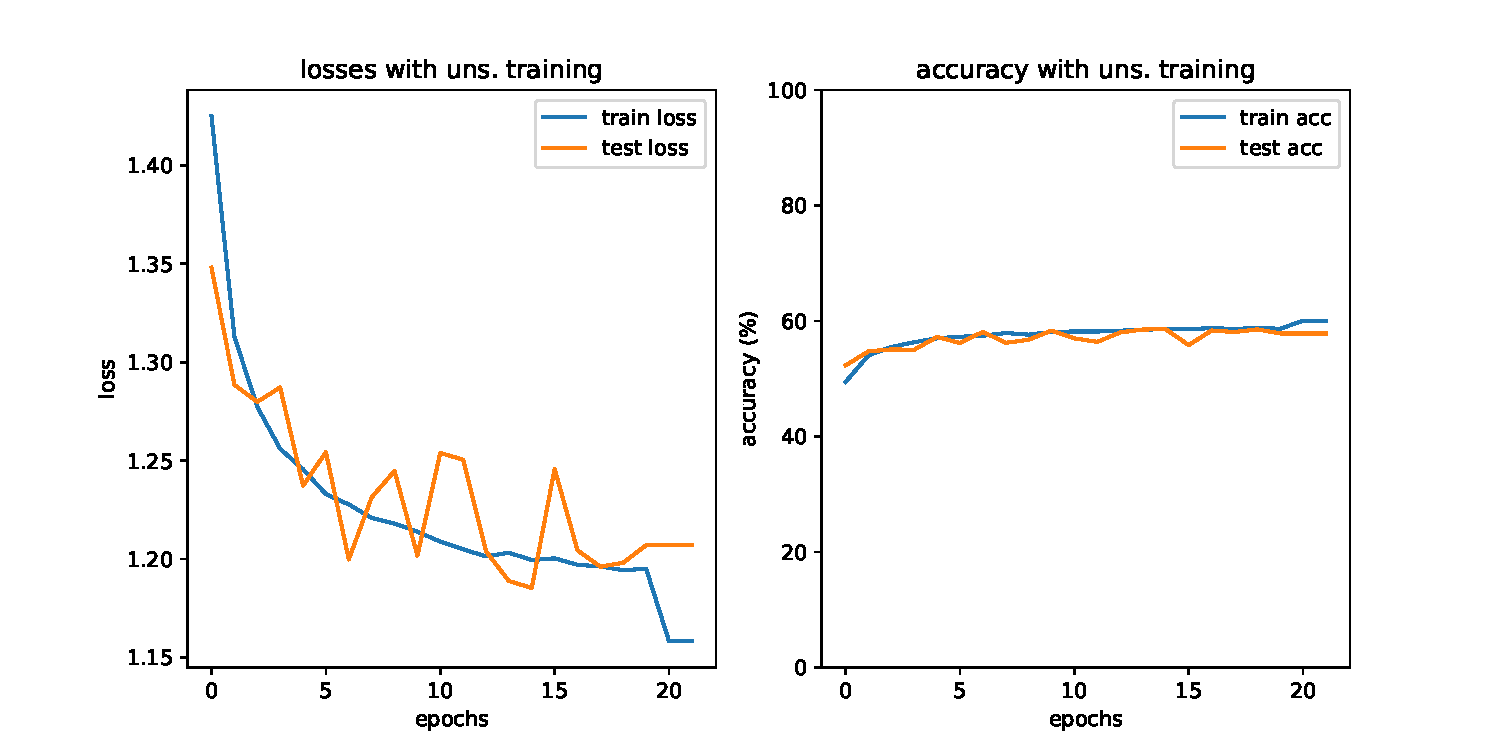
\includegraphics[width=1.2\textwidth]{linear_classif_occ_cifar10.pdf}
  \caption{linear classsification with occlusions - cifar10}
  \label{fig:linear classsification with occlusions - cifar10 }
\end{figure}

In linear classification with occlusions, the input data is intentionally modified by introducing occlusions or partial obscuring of the features. This can have an impact on the performance and behavior of the classifier compared to the normal linear classification without occlusions. 

The second subplot presents the training and testing accuracy. The accuracy values are similar to the linear classification graph, indicating that the model's classification performance remains consistent throughout training.

The high similarity between the graphs of linear classification with occlusions and without occlusions can be attributed to robust features that remain unaffected by occlusions, occlusion patterns that do not significantly alter the data distribution, and adequate training of the classifier to handle occluded data. These factors enable the classifier to extract relevant features, maintain accurate predictions, and exhibit similar performance and trends in both scenarios.

\subsubsection{Confusion Matrix}
\begin{figure}[H]
 \centering
  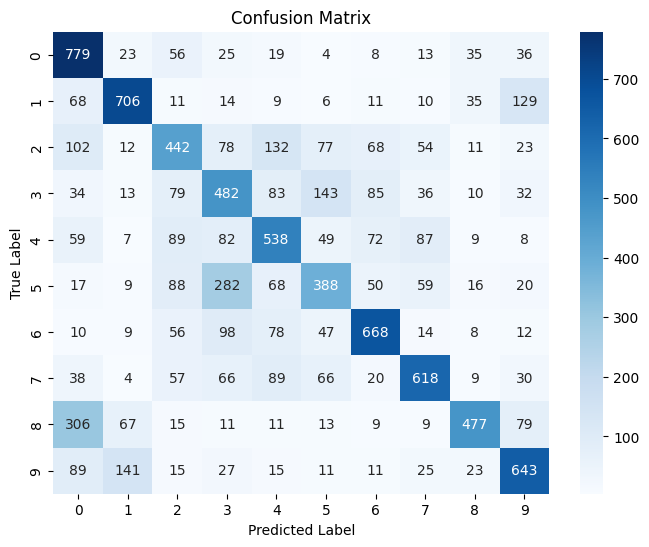
\includegraphics[width=0.9\textwidth]{confusion_matrix_cifar10.png}\hfill
  \label{fig: confusion matrix - cifar10}
\end{figure}

The graph shows a confusion matrix, which is a visual representation of the model's performance in predicting the true labels versus the predicted labels.
The rows of the matrix represent the true labels, while the columns represent the predicted labels. Each cell in the matrix indicates the count of instances where a true label corresponds to a predicted label.

From the confusion matrix, you can observe the following:
\begin{itemize}
  \item Labels 0, 1, 8, and 9 are predicted accurately with relatively high counts, suggesting good performance for these classes.
  \item However, there are instances of misclassifications, such as label 5 being predicted as 3 for 282 times and label 8 being predicted as 0 for 306 times.
  \item These errors indicate that the model may struggle to differentiate between certain latent variables, leading to confusion between similar classes.
  
It's important to further analyze the specific characteristics and patterns of the misclassified classes to identify potential reasons for the errors. This analysis can help in improving the model's performance by addressing the challenges associated with distinguishing between certain latent variables.
\end{itemize}

\subsection{Evaluation - SVHN}
\subsubsection{Linear Classification}
\begin{figure}[H]
  \centering
  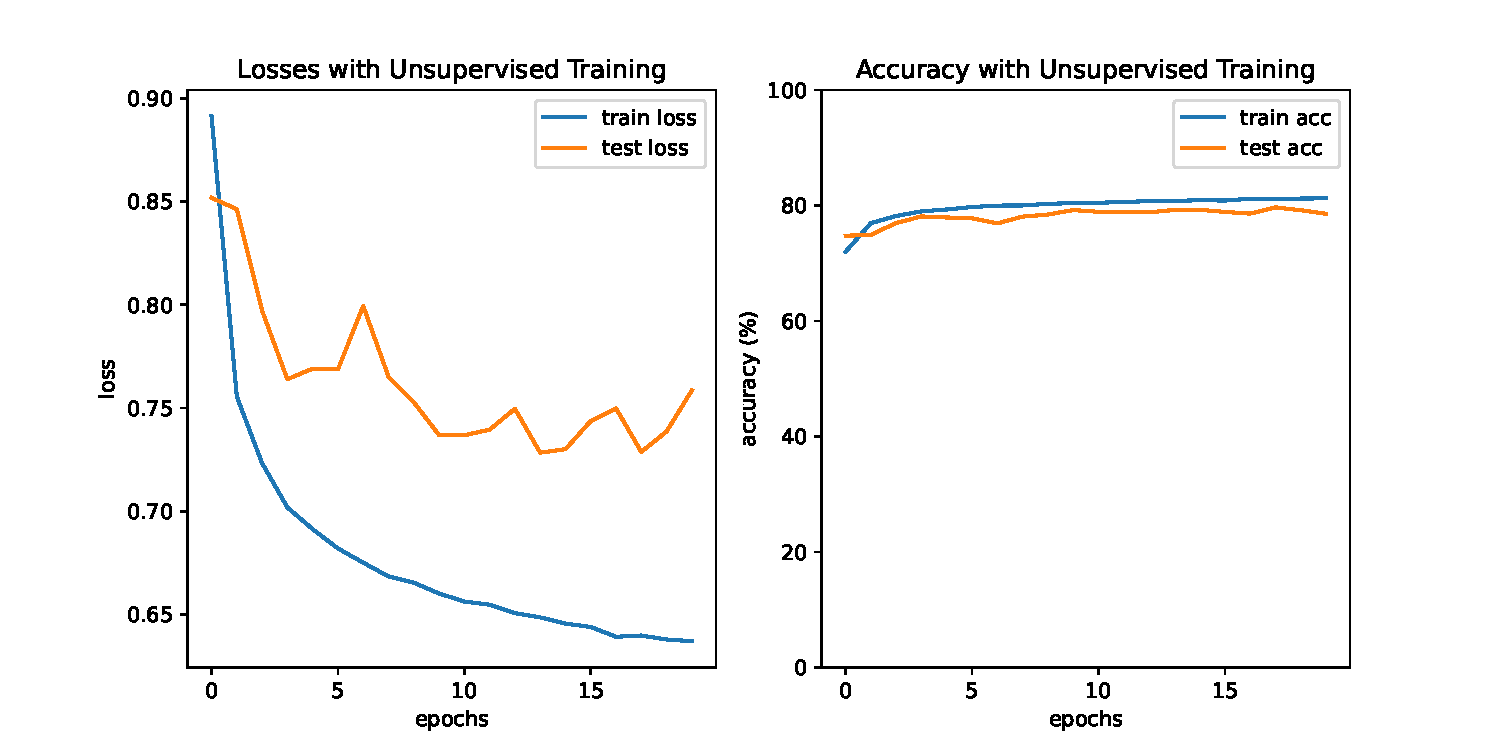
\includegraphics[width=1.2\textwidth]{linear_classif_svhn.pdf}
  \caption{linear classification - svhn}
  \label{fig:linear classification - svhn}
\end{figure}
The first subplot displays the training and testing losses over the epochs. The train loss consistently decreases over time, indicating that the model is learning and improving its performance on the training data. However, the test loss fluctuates and remains generally higher than the train loss, suggesting that the model may not generalize well to unseen data.

The second subplot shows the training and testing accuracies over the epochs. Both the train and test accuracies remain consistently around 80\%, indicating that the model is able to classify the data with a relatively high accuracy. However, it's important to note that the accuracy alone may not provide a complete picture of the model's performance, as the test loss suggests potential overfitting or lack of generalization ability.

The consistent decrease in train loss and stable accuracy on both train and test sets indicate that the model is successfully learning from the training data. However, the fluctuating test loss and the fact that it remains higher than the train loss suggest that the model might be overfitting to the training data and struggling to generalize well to unseen data. 



\subsubsection{Losses}
\begin{figure}[H]
  \centering
  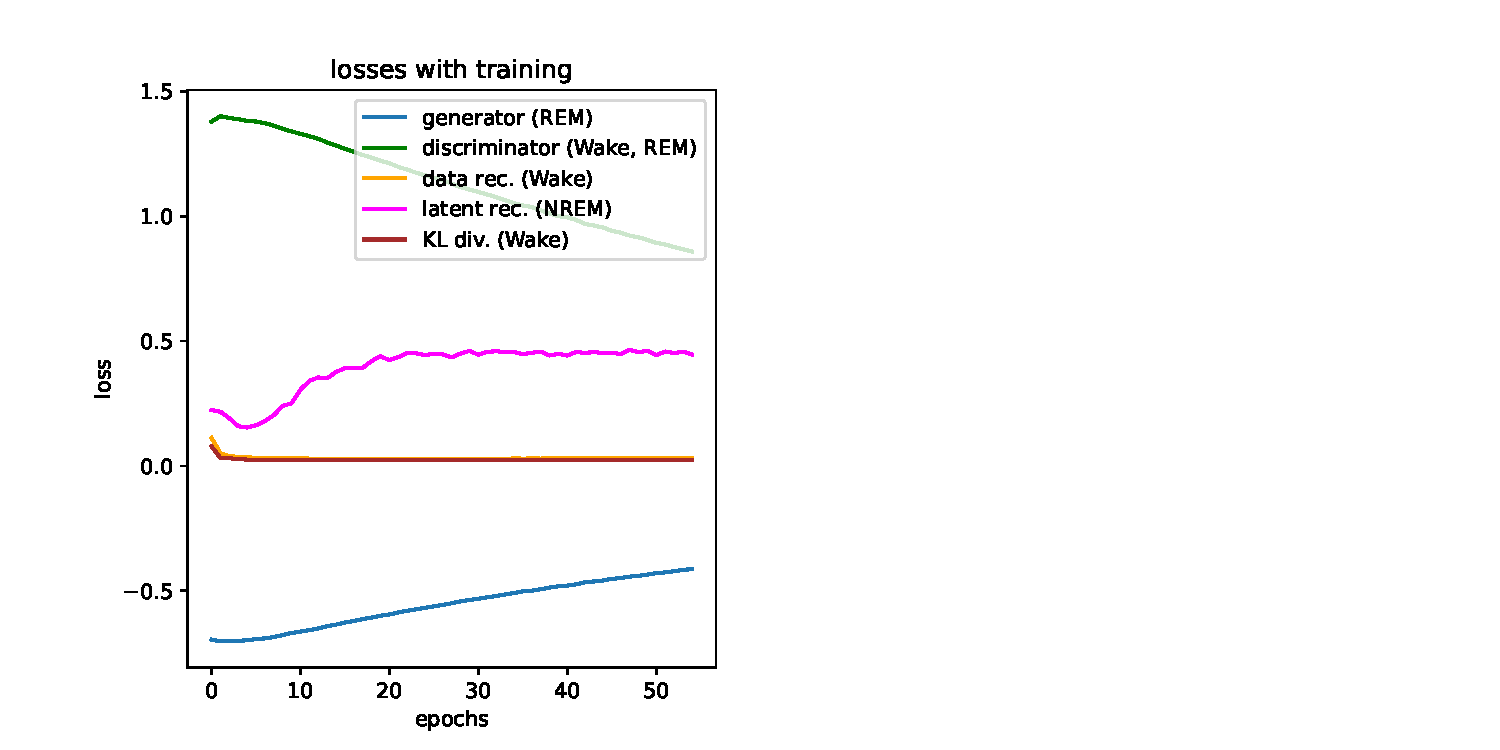
\includegraphics[width=1.2\textwidth]{losses_svhn.pdf}
  \caption{losses - svhn}
  \label{fig:losses - svhn}
\end{figure}
The discriminator loss (associated with both Wake and REM sleep) decreases from an initial value of 1.5 to approximately 1.0 over the epochs. This indicates that the discriminator is becoming more proficient at distinguishing between real and generated data. The losses for data reconstruction (associated with Wake) and latent reconstruction (associated with NREM) remain relatively stable.  Both losses hover around 0.0, suggesting that the model is consistently able to reconstruct the input data accurately.

Overall, the decreasing discriminator loss and stable reconstruction losses suggest that the model is effectively learning and improving its performance in different aspects of the training process. The stable KL divergence loss indicates that the model is successfully matching the latent distribution to the prior. The floating NREM loss may indicate some variation in the model's ability to reconstruct the latent data associated with NREM sleep. 




\subsubsection{Occlusions}
\begin{figure}[H]
  \centering
  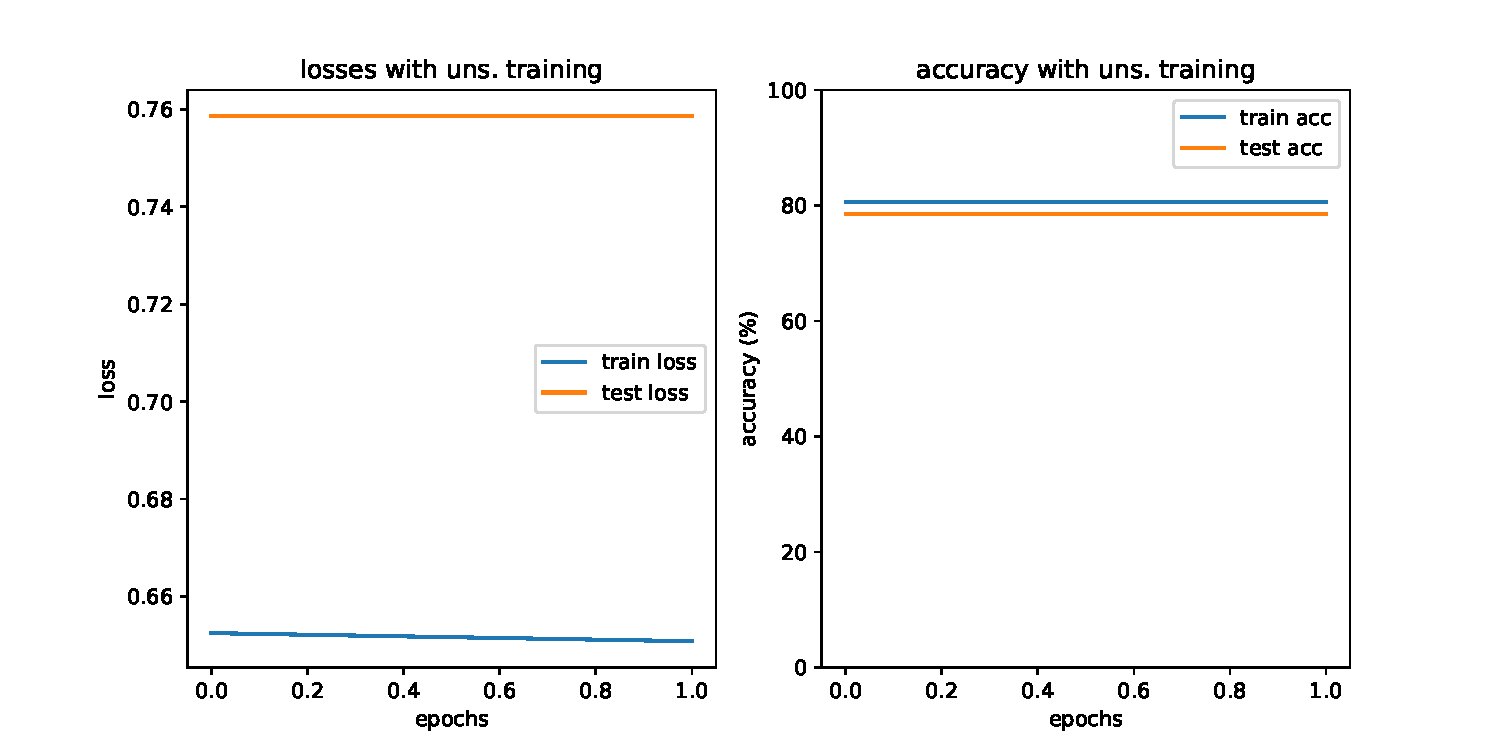
\includegraphics[width=1.2\textwidth]{linear_classif_occ_svhn.pdf}
  \caption{linear classification with occlusions - svhn}
  \label{fig:linear classification with occlusions - svhn}
\end{figure}
The training loss (blue line) remains stable around 0.6 from the beginning to the end of training. This indicates that the model is consistently able to minimize the loss on the training data, suggesting a good fit to the training set. The testing loss (orange line) also remains stable around 0.75 throughout the training process. This suggests that the model's performance on unseen data, represented by the testing set, is relatively consistent. The stable losses for both training and testing indicate that the model is not overfitting or underfitting the data.

The second subplot displays the training and testing accuracies over the epochs. The training accuracy (blue line) remains around 80\% throughout the training process. This indicates that the model is consistently able to classify the training data correctly with a relatively high accuracy. Similarly, the testing accuracy (orange line) also remains around 80\% throughout the training process, indicating that the model's performance on unseen data is consistent with its performance on the training data.

Overall, the stable losses and accuracies for both training and testing suggest that the model has reached a certain level of performance and is not improving significantly further. This may indicate that the model has converged and has learned to capture the patterns and relationships present in the data. 

\subsubsection{Confusion Matrix}
\begin{figure} [H]
 \centering
  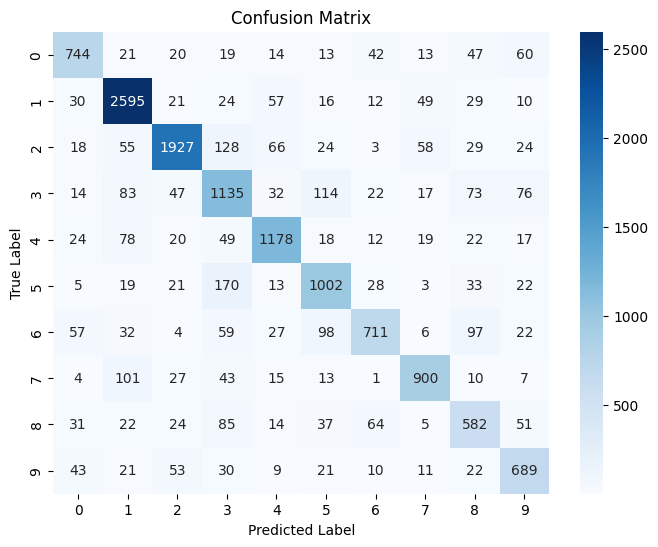
\includegraphics[width=0.9\textwidth]{confusion_matrix_svhn.png}\hfill
\end{figure}
In the given confusion matrix, the model's performance appears to be quite accurate overall. Here are some observations based on the provided information:
The diagonal cells represent the correct predictions, where the true label matches the predicted label. For example, there are approximately 2595 observations from label 1 that were correctly classified.

The off-diagonal cells represent the misclassifications. For instance, the cell where true label 5 and predicted label 3 intersect indicates that there were 170 instances where observations from label 5 were misclassified as label 3.
Similarly, the cell where true label 3 and predicted label 5 intersect indicates that there were 114 instances where observations from label 3 were misclassified as label 5.
Overall, a high count on the diagonal and low counts in the off-diagonal cells suggest good performance of the classifier. 






\subsection{Evaluation - MNIST}
\subsubsection{Linear Classification}
\begin{figure}[H]
  \centering
  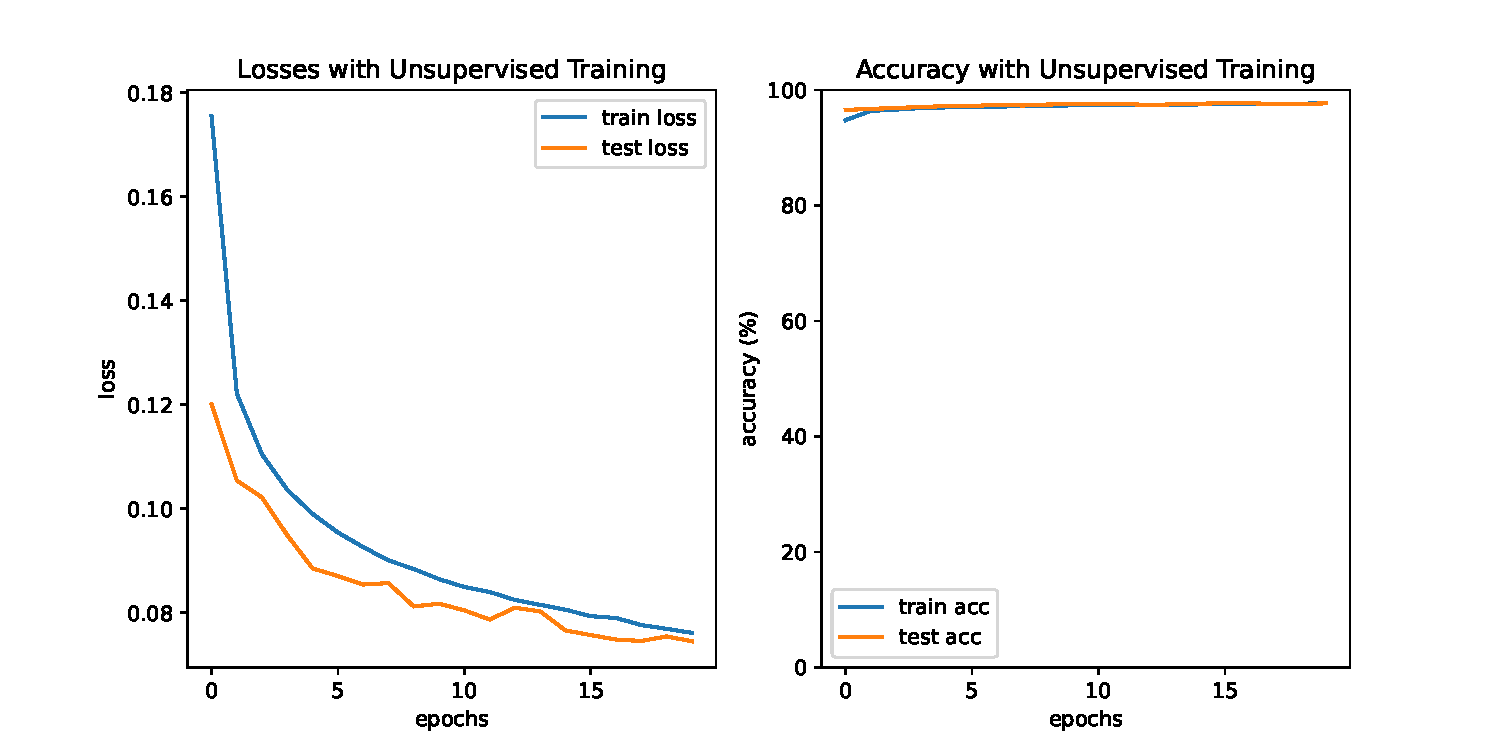
\includegraphics[width=1.2\textwidth]{linear_classif_mnist.pdf}
  \caption{linear classification - mnist}
  \label{fig:linear classification - mnist}
\end{figure}
In the loss plot, both the training and test loss curves exhibit a similar trend. Starting at around 0.18, the losses gradually decrease over the course of the training process. By the end, they reach approximately 0.08. This suggests that the model effectively learns from the data and improves its predictive capabilities.

The accuracy plot reveals consistent and high accuracy levels throughout the training. Both the training and test accuracy curves remain stable at around 98\% from the beginning to the 20th epoch. This indicates that the model performs well not only on the training data but also on unseen test data, demonstrating its ability to generalize and make accurate predictions.

Overall, the graph demonstrates that the linear classifier achieves low loss values and high accuracy rates during the training phase. These results signify that the classifier has effectively learned meaningful representations and can accurately classify the input data.

\subsubsection{Losses}
\begin{figure}[H]
  \centering
  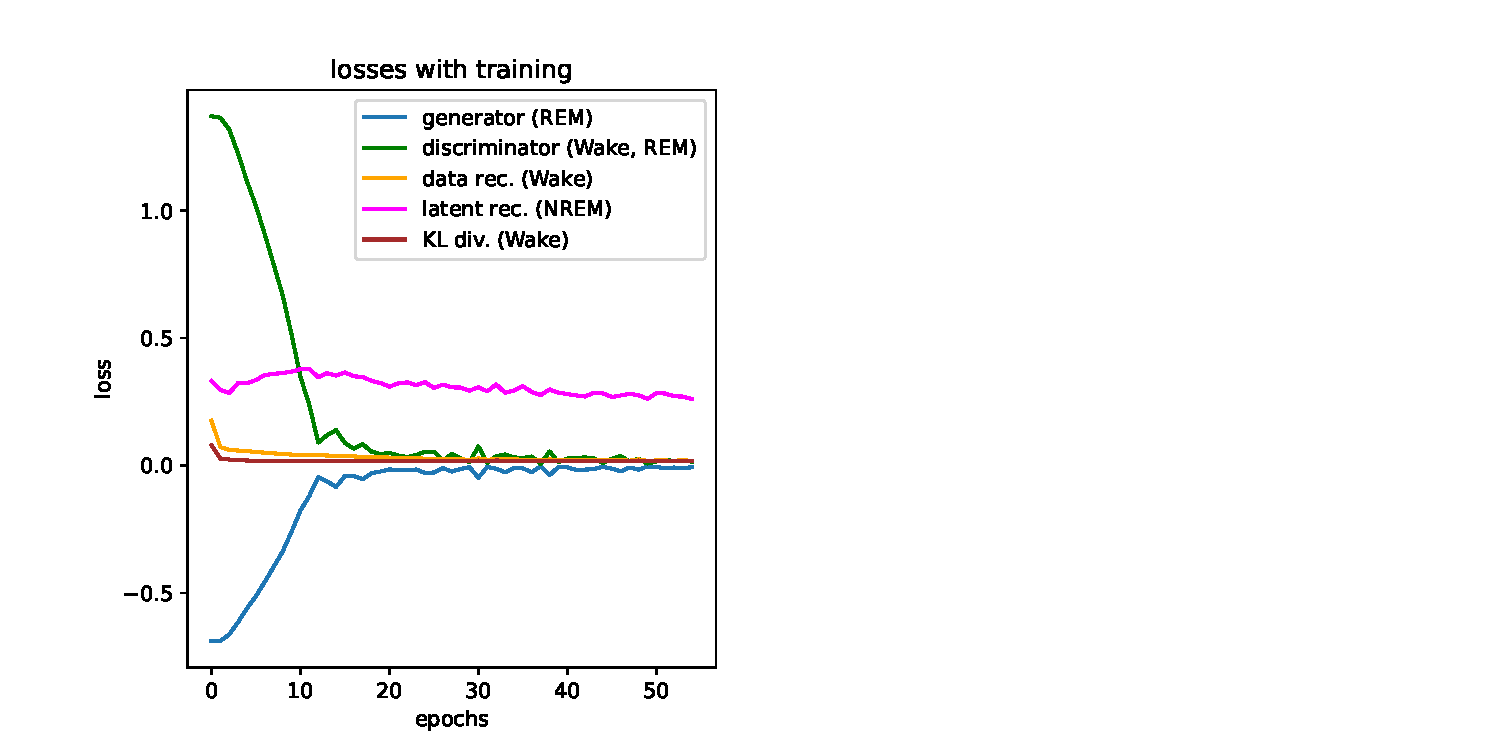
\includegraphics[width=1.2\textwidth]{losses_mnist.pdf}
  \caption{losses - mnist}
  \label{fig: losses - mnist}
\end{figure}
The discriminator losses show a significant decrease from 1.5 to 0.2 after the 10th epoch, remaining relatively stable thereafter. This suggests that the discriminator is effectively learning to differentiate between the target classes (Wake and REM sleep).

The data reconstruction losses for the wake state and the KL divergence losses exhibit similar curves, both hovering around 0.0 throughout the training. This indicates that the model successfully reconstructs the input data in the wake state and effectively minimizes the KL divergence, which is a measure of the dissimilarity between distributions.

In contrast, the generator losses show an increase in loss at the same time the discriminator experiences a significant downgrade. This observation suggests an interplay between the generator and discriminator during training, where the generator faces a more challenging task when the discriminator becomes more proficient at distinguishing between classes.

\subsubsection{Occlusions}
\begin{figure}[H]
  \centering
  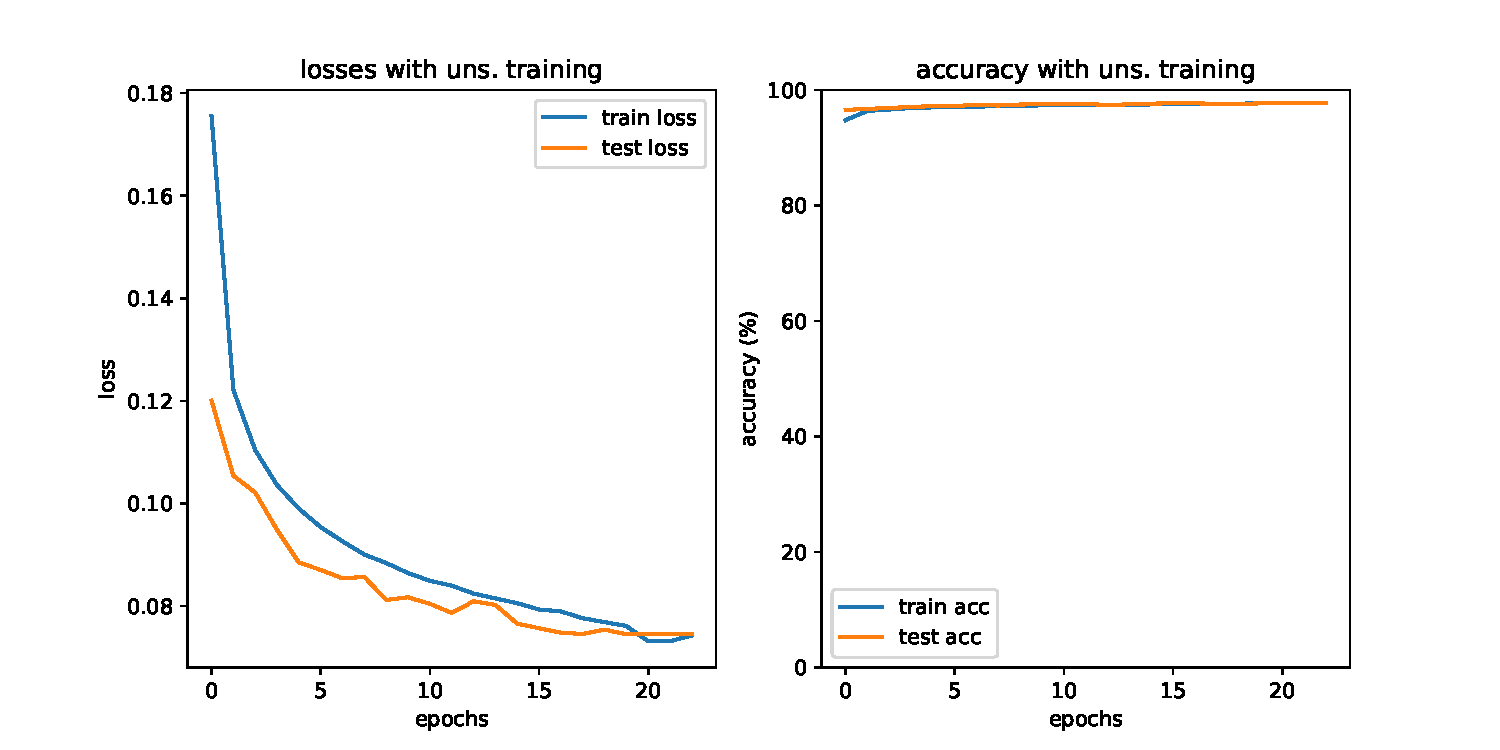
\includegraphics[width=1.2\textwidth]{linear_classif_occ_mnist.pdf}
  \caption{linear classification with occlusions - mnist}
  \label{fig: linear classification with occlusions - mnist}
\end{figure}
Both the training and testing losses for normal observations and observations with occlusions follow similar curves. This indicates that the linear classifier performs consistently well in terms of minimizing the loss for both types of data. The similar loss curves suggest that the occlusions in the observations do not significantly impact the performance of the linear classifier.

The right subplot depicts the accuracies (training and testing) over the epochs. Again, the accuracy curves for normal observations and observations with occlusions are almost identical. This implies that the linear classifier achieves similar levels of accuracy in correctly classifying both types of data. The presence of occlusions does not seem to hinder the classifier's ability to make accurate predictions.

Overall, the graph suggests that the linear classifier is robust to occlusions and maintains its performance in terms of both loss minimization and accuracy. This indicates that the linear classifier is capable of effectively handling data with occlusions and can generalize well to different types of observations.


\subsubsection{Confusion Matrix}
\begin{figure}
\centering
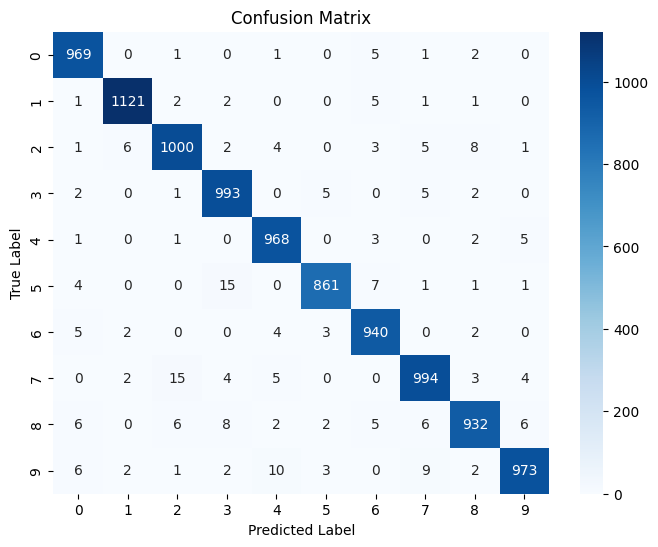
\includegraphics[width=0.9\textwidth]{confusion_matrix_mnist.png}\hfill
\end{figure}
It seems that the confusion matrix shows a strong diagonal pattern, indicating that the majority of the predictions match the true labels. This suggests that the linear classifier is performing well in correctly classifying the test data. The fact that there are only a few instances misclassified (less than 20 times) for various variables indicates a high level of accuracy in the classification.
For example, the statement out of 1133 instances of class 1, the classifier correctly predicted 1121 instances as class 1 and misclassified only 12 instances. This further supports the conclusion that the linear classifier is accurate and has a strong performance.
Overall, the confusion matrix demonstrates that the linear classifier has achieved a high level of accuracy and is capable of effectively distinguishing between different classes in the test data.






\subsection{Evaluation - FASHION}
\subsubsection{Linear Classification}
\begin{figure}[H]
  \centering
  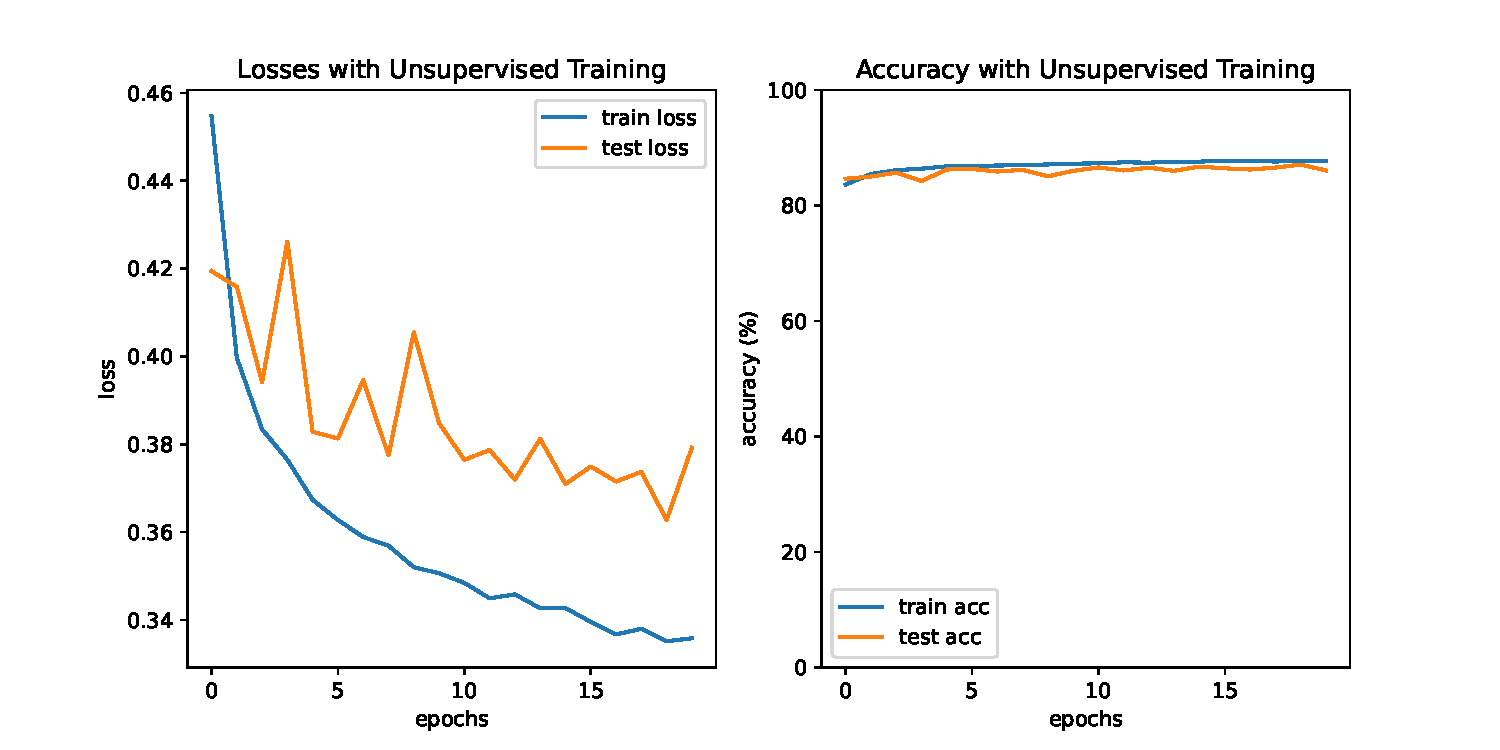
\includegraphics[width=1.2\textwidth]{linear_classif_fashion.pdf}
  \caption{linear classification - fashion}
  \label{fig:linear classification - fashion}
\end{figure}
It is observed that the training loss steadily decreases from approximately 0.46 to less than 0.34 over 20 epochs. On the other hand, the test loss shows more fluctuations and variations, starting at 0.42 and ending at around 0.39. This suggests that the model is learning from the training data and gradually improving its performance, but the test loss fluctuates due to the model's ability to generalize to unseen data.

The accuracy starts and ends around 82\%, indicating that the model achieves a reasonably high level of accuracy in classifying the data.

Overall, the graphs demonstrate that the linear classifier is learning and improving its performance over the epochs of unsupervised training. The decreasing training loss suggests that the model is effectively capturing patterns and reducing errors on the training data. However, the fluctuating test loss indicates that the model's performance on unseen data may not be as consistent. 


\subsubsection{Losses}
\begin{figure}[H]
  \centering
  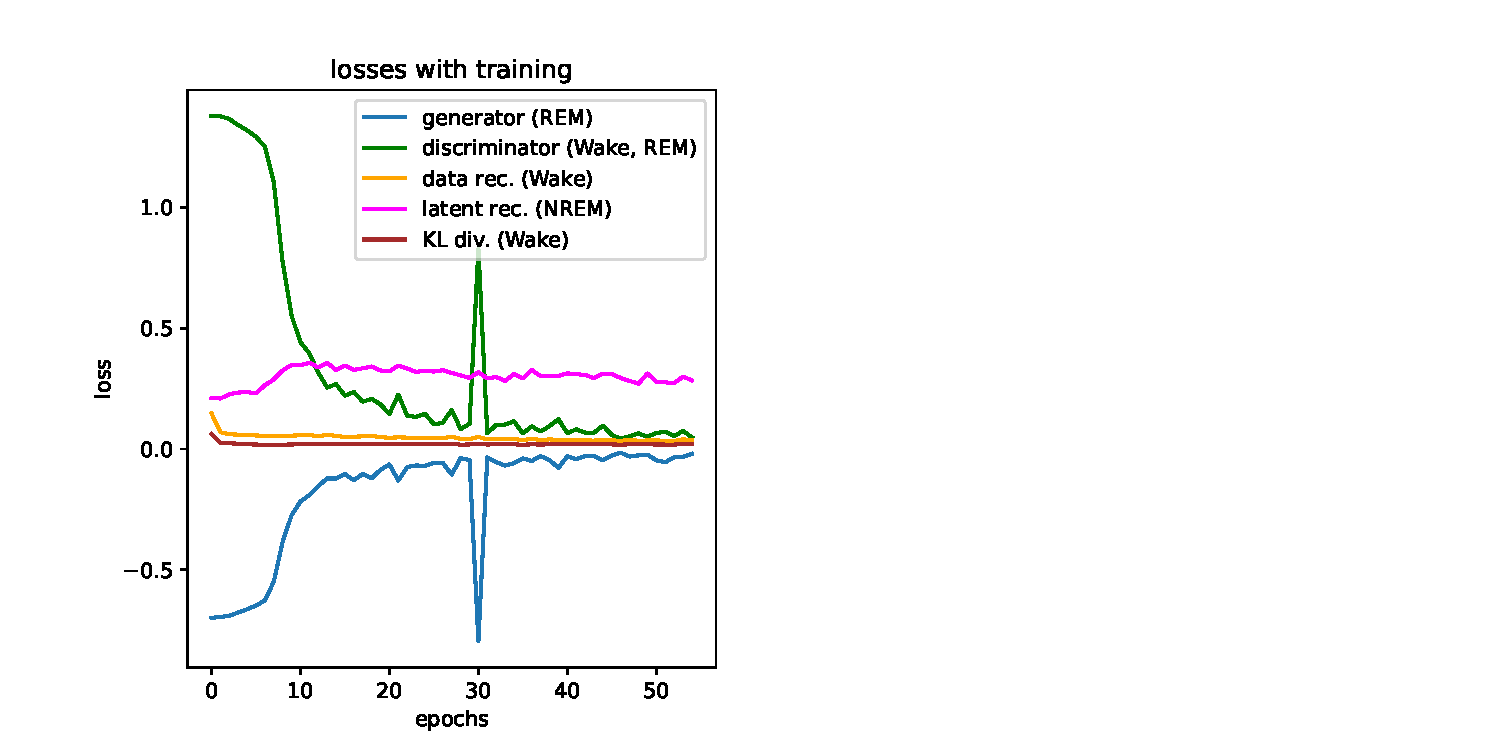
\includegraphics[width=1.2\textwidth]{losses_fashion.pdf}
  \caption{losses - fashion}
  \label{fig:losses - fashion}
\end{figure}
At around 10 epochs, there is a significant decrease in the loss of the discriminator (green line), while the loss of the generator (blue line) experiences a sharp increase. This indicates that, during this period, the discriminator is becoming more effective at differentiating between the Wake and REM phases, while the generator faces challenges in generating realistic REM data. As a result, the generator adjusts its parameters to improve the quality of generated REM data, which leads to an increase in its loss.

Subsequently, at around 30 epochs, there is another notable change in the losses. The discriminator's loss increases, indicating that it struggles to distinguish between the Wake and REM phases, while the generator's loss decreases, suggesting that it successfully generates more realistic REM data. This pattern suggests a dynamic competition between the generator and discriminator, with each trying to outperform the other.


\subsubsection{Occlusions}
\begin{figure}[H]
  \centering
  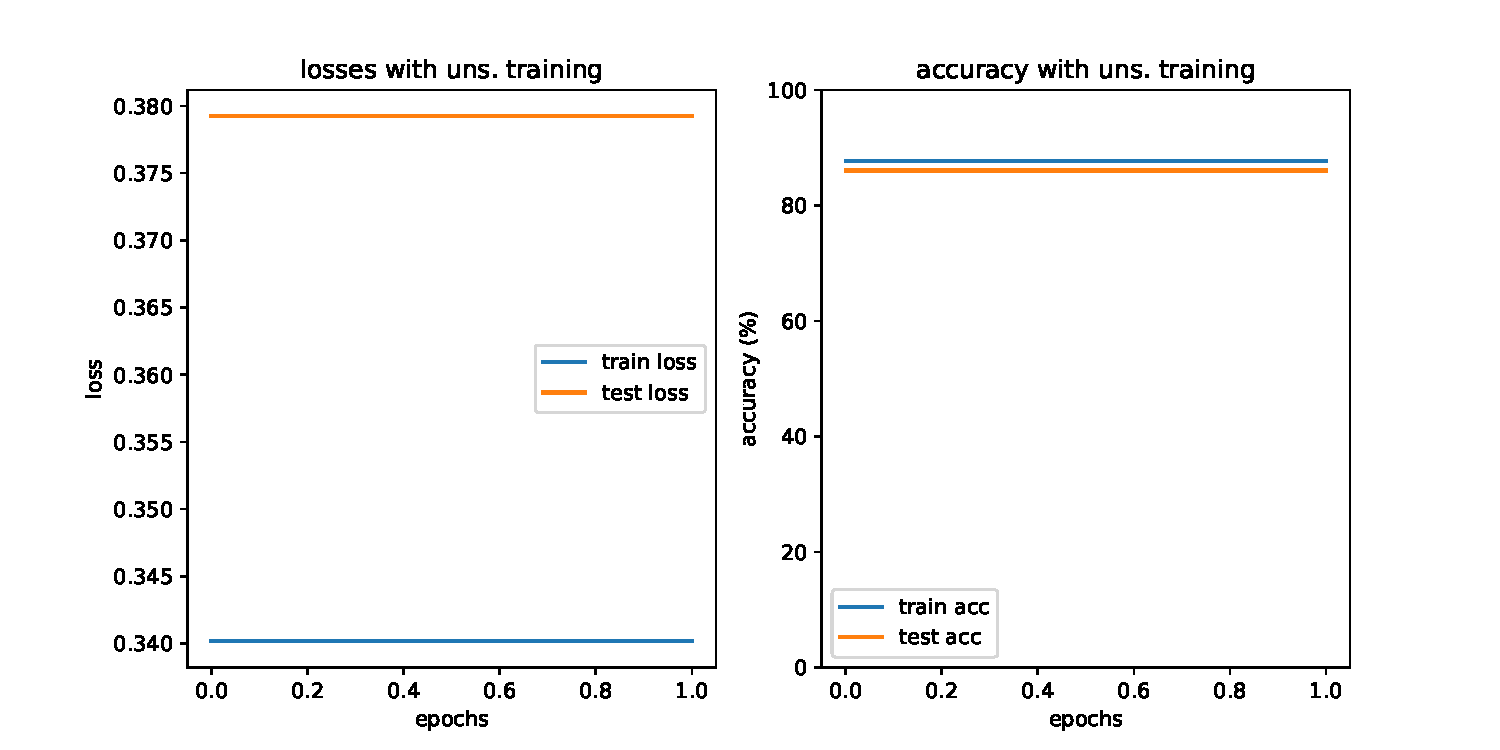
\includegraphics[width=1.2\textwidth]{linear_classif_occ_fashion.pdf}
  \caption{linear classification with occlusions - fashion}
  \label{fig:pdf-image}
\end{figure}
The training loss starts and finishes at approximately 0.370, while the testing loss starts and finishes at around 0.340. The stability and similarity between the training and testing losses indicate that the model is not overfitting to the training data and is performing consistently on unseen testing data.

The training accuracy with occlusions starts and finishes at around 84\%, while the testing accuracy starts and finishes at approximately 83\%. The similarity in performance between the training and testing accuracies indicates that the model generalizes well to unseen data and is not over-reliant on the training set.

Overall, the graph demonstrates that the linear classifier model achieves stable and consistent performance throughout the training process. 


\subsubsection{Confusion Matrix}
\begin{figure}[H]
\centering
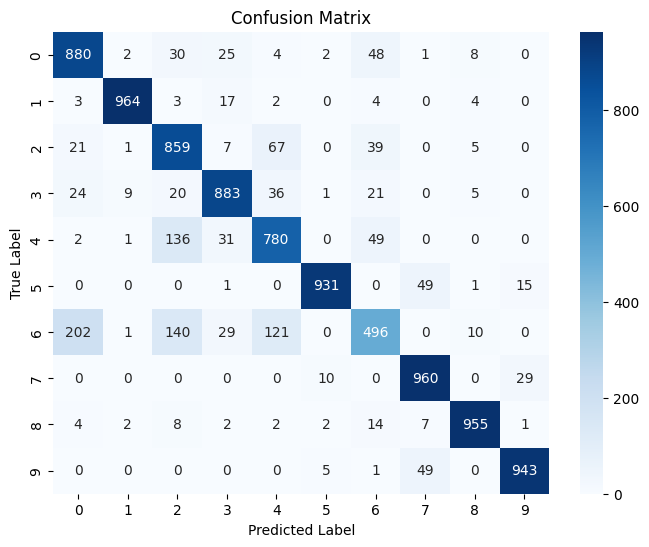
\includegraphics[width=0.9\textwidth]{confusion_matrix_fashion.png}\hfill
\end{figure}
Based on the confusion matrix, it appears that class 6 has the most mismatches. It has been misclassified as class 0, 2, and 4. This suggests that the model is having difficulty distinguishing class 6 from these other classes. On the other hand, class 6 has the lowest percentage of correct matches, indicating that the model's performance is relatively poorer for this particular class.


\section{Conclusions}
In this study, we have explored the relationship between dreams, semantic representations, and the evolutionary process. The article model of cortical representation learning emphasizes the role of dreams in the creative development of episodic memories, contributing to the acquisition of semantic representations. By analyzing four distinct datasets using a cortical architecture inspired by generative adversarial networks (GANs), we have uncovered the profound impact of dream-driven episodic memories on semantic representations. These findings provide insights into dream-inspired learning mechanisms and have broader implications for understanding sensory learning in humans and other organisms. In this concluding chapter, we present our key findings and discuss the significance of dreams in shaping the representation of sensory experiences in the brain.

\begin{enumerate}
 
 \item Dream-Driven Episodic Memory Formation: The proposed functional model of cortical representation learning, inspired by generative adversarial networks (GANs), reveals a significant link between dreams and the formation of semantic representations. By creatively developing episodic memories, dreams play a fundamental role in shaping the brain's ability to generate meaningful and contextually rich representations of sensory experiences, thereby contributing to the evolutionary process.

 \item Semantic Representations Enriched by Dream-Induced Memories: Through training the cortical architecture using established datasets of natural images, the study demonstrates that the acquisition of high-quality semantic representations is greatly influenced by the incorporation of dream-induced memories. This finding underscores the evolutionary advantage of dreams in enhancing the brain's capacity to form rich and nuanced representations that go beyond direct sensory input.

 \item Unveiling Dream-Inspired Learning Mechanisms: The insights gained from the proposed cortical model shed light on the underlying mechanisms through which dreams aid in the formation of semantic representations. By simulating the creative and integrative processes observed in dreams, the model replicates the brain's ability to consolidate and generalize sensory experiences, providing a glimpse into the evolutionary significance of dream-driven learning mechanisms.

 \item Implications for Understanding Learning from Sensory Input: The research findings extend beyond the realm of dreams and offer profound implications for comprehending how humans and other organisms learn from sensory input. By revealing the role of dreams in the formation of semantic representations, this study illuminates an additional layer of complexity in the learning process, emphasizing the importance of holistic, creative, and contextually informed representations in adapting to the environment and facilitating knowledge acquisition throughout evolution.
\end{enumerate}

\end{document}


\end{document}




